\chapter{Introducción a los sistemas de protección}
\section{Defectos eléctricos}
\begin{table}[H]
	\centering
	\renewcommand{\arraystretch}{1.5} % Espaciado entre filas
	\setlength{\tabcolsep}{5pt} % Espaciado horizontal en celdas
	\begin{tabular}{|p{3cm}|p{3cm}|p{3cm}|p{3cm}|}
		\hline
		\textbf{Causas}                           & \textbf{Cortocircuito}                & \textbf{Sobrecarga}                 & \textbf{Sobretensión}           \\ \hline
		Factores atmosféricos y climáticos        & Rayos, Hielo, Viento, Humedad         & Rayos, Hielo, Viento, Humedad       & Rayos                          \\ \hline
		Influencia de animales y vegetación       & Aves, Roedores, Árboles              & Aves, Roedores, Árboles            & ---                            \\ \hline
		Envejecimiento del material               & Falta aislamiento                    & Falta aislamiento                  & ---                            \\ \hline
		Fallos electromecánicos                   & Fallo equipos, Defecto material      & Agarrotamientos                    & Anormalidad de equipos         \\ \hline
		Factores humanos                          & Grúas, Errores operación             & Utilización inadecuada             & Errores de operación           \\ \hline
	\end{tabular}
\end{table}
\section{Sistema de protección básico}
\begin{figure}[H]
	\centering
	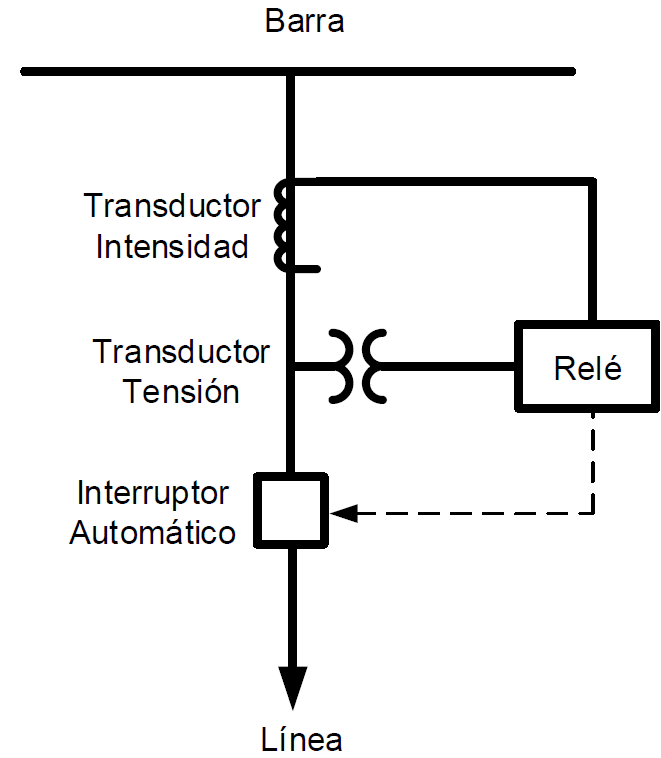
\includegraphics[width=0.3\linewidth]{Images/42}
	\label{fig:42}
\end{figure}

Se define el relé de protección como un dispositivo que provoca el cambio brusco en uno o varios circuitos de control cuando la magnitud vigilada cambia de una manera determinada. Tiene distintas funciones de protección según la magnitud vigilada.
\begin{itemize}
	\item Tensión
	\begin{itemize}
		\item Sobretensión
		\item Tensión mínima
		\item Tensión
	\end{itemize}
	\item Intensidad
	\begin{itemize}
		\item  Sobreintensidadde tiempo inverso
		\item Sobreintensidadde tiempo fijo
		\item Sobreintensidaddireccional
	\end{itemize}
	\item Potencia
	\begin{itemize}
		\item  Potencia
		\item Potencia direccional
	\end{itemize}
	\item Diferenciales
	\begin{itemize}
		\item Relés diferenciales de barras
		\item Relés diferenciales de transformador
	\end{itemize}
	\item Impedancia: Relés de impedancia = Relés de distancia
	\item Frecuencia: Relés de frecuencia
	\item Temperatura: Relés de temperatura
\end{itemize}
\subsection{Parámetros principales}
\begin{itemize}
	\item \textbf{Tiempo de respuesta}: Tiempo desde que se produce el defecto hasta que el relé conmuta sus contactos de aviso o disparo del disyuntor
	\item \textbf{Relación de reposición ( R )}: Relación entre el valor real de la magnitud que desactiva el relé y el valor para el que se activa
	\begin{itemize}
		\item Relés de valor máximo: $0 < R \ge 1$
		\item Relés de valor mínimo: $1 \ge R < \infty$
	\end{itemize}
	\item \textbf{Histéresis de conexión 1 / R}:
	\item \textbf{Tiempo de reposición}: Tiempo que se necesita para que el relé después de operar vuelva de nuevo a las condiciones iniciales
\end{itemize}
\subsection{Función interruptores automáticos de alta tensión}
\begin{itemize}
	\item Cerrar, soportar y abrir corrientes de cortocircuito
	\item Poder de cierre y poder de corte
	\item También se denominan disyuntores
	\item La apertura automática se realiza a través de relés de protección
\end{itemize}
\section{Componentes y esquemas de Alta Tensión}
\begin{itemize}
	\item Alimentación única: protecciones en el inicio de línea
	\item Alimentación doble: Protecciones en ambos extremos de línea. La intensidad de falta se aporta desde ambos extremos
\end{itemize}
\begin{figure}[H]
	\centering
	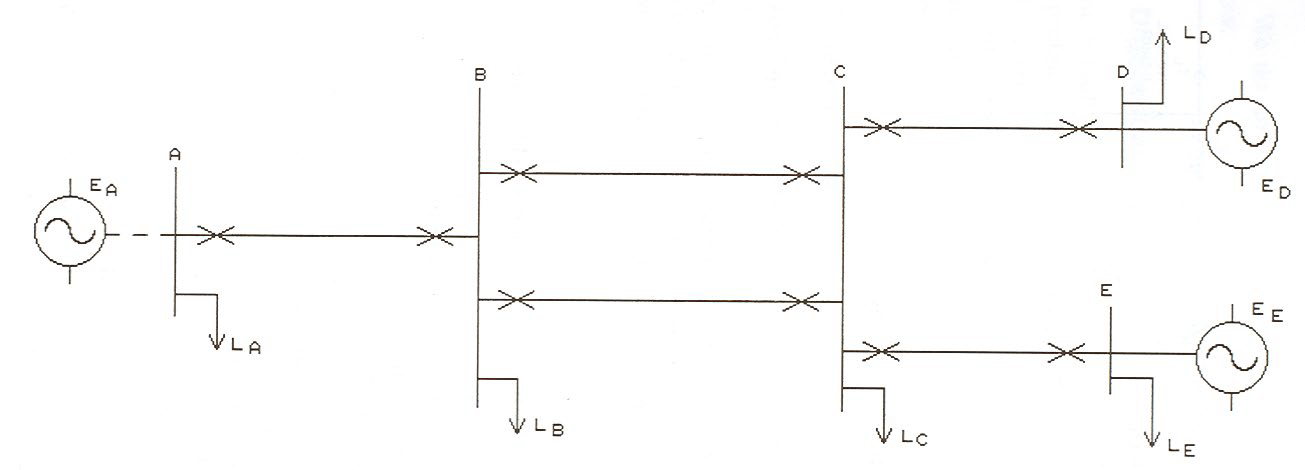
\includegraphics[width=0.7\linewidth]{Images/43}
	\label{fig:43}
\end{figure}

\begin{figure}[H]
	\centering
	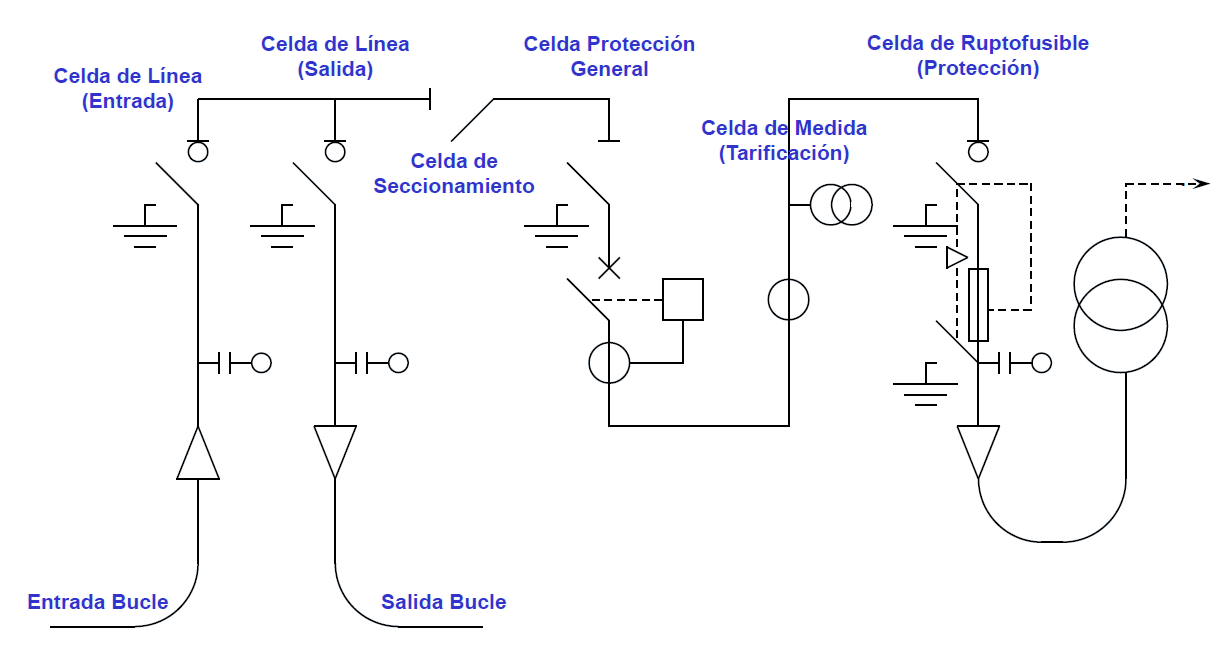
\includegraphics[width=0.7\linewidth]{Images/44}
	\label{fig:44}
\end{figure}


\section{Zonas de protección}
Se define como la parte de la red que debe quedar aislada cuando en el interior de la misma se produce un defecto. Incluye el elemento o elementos protegidos más los interruptores automáticos que conectan dicho elemento al resto del sistema eléctrico. Las zonas de protección deben estar “solapadas” para que no queden zonas de la red sin proteger.
\begin{figure}[H]
	\centering
	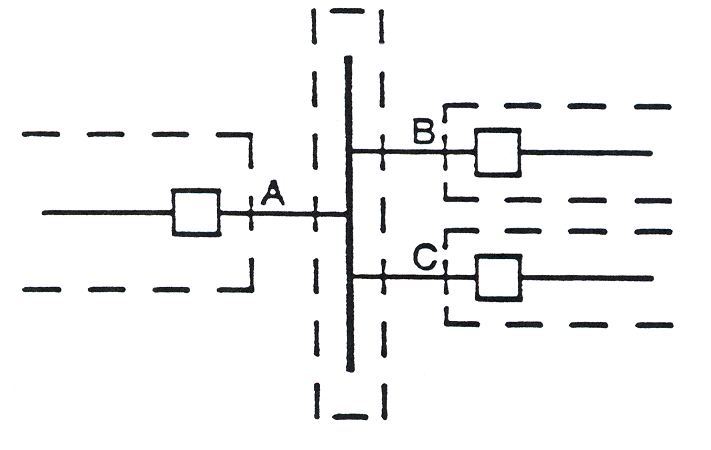
\includegraphics[width=0.5\linewidth]{Images/45}
	\label{fig:45}
\end{figure}
\begin{figure}[H]
	\centering
	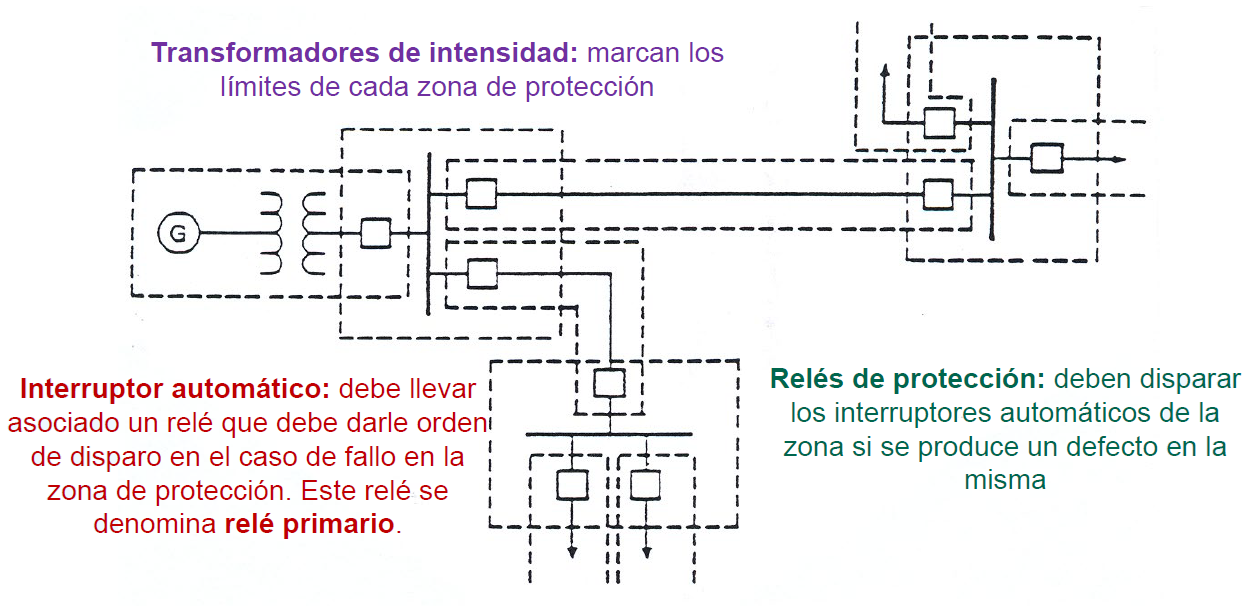
\includegraphics[width=0.7\linewidth]{Images/46}
	\label{fig:46}
\end{figure}
\begin{itemize}
	\item La función de protección más selectiva y rápida del relé primario es la función de protección principal
	\item El resto de funciones se denominan “complementarias” que son menos selectivas y menos rápidas
\end{itemize}
\subsection{Respaldo remoto}
Protección de respaldo que produce la apertura de un interruptor automático de otra subestación. Interruptores en cascada.
\subsection{Respaldo local}
Protección situada en la misma zona de protección. Dos posibilidades:
\begin{itemize}
	\item Situada en la misma posición que la protección principal:
	\begin{itemize}
		\item Se suelen duplicar los núcleos de los transformadores de protección y los circuitos de disparo de los interruptores automáticos
		\item Puede ser idéntica a la protección primaria o integrar relés con otras funciones
	\end{itemize}
	\item Disparo de interruptores automáticos adyacentes al interruptor que no dispara
\end{itemize}
\section{Identificación de dispositivos de corte y protección}
\begin{table}[H]
	\centering
	\begin{tabular}{|c|c|c|}
		\hline
		\textbf{ANSI} & \textbf{IEC} & \textbf{Dispositivo} \\ \hline
		27 & $U<$ & Relé de mínima tensión ac \\ \hline
		50 & $I>$, $I>>$ & Relé de sobreintensidad de tiempo fijo \\ \hline
		50N & $IE>$, $IE>>$ & Relé de sobreintensidad de tiempo fijo de fallo a tierra \\ \hline
		51 & $I>t$, $I>>t$ & Relé de sobreintensidad de tiempo inverso \\ \hline
		51N & $IE>t$, $IE>>t$ & Relé de sobreintensidad de tiempo inverso de fallo a tierra \\ \hline
		59 & $U>t$, $U>>t$ & Relé de sobretensión ac \\ \hline
	\end{tabular}
	\label{tab:protection_devices}
\end{table}